\paragraph{Justification de la modélisation choisie}

\subparagraph{Machine 1: envoi des wagons par le biais d'un buffer}

La première machine se découpe comme suit. Tout d'abord, nous avons créé un
tableau ``tabVoie'' qui prend des indices compris entre 1 et ``nbWagons'',
constante définie dans le contexte c1, appartenant aux entiers positifs
supérieurs à 0, et retourne un champ appartenant à ``TOWN''. Cette dernière
est une partition. C'est-à-dire que sa valeur est l'un des deux champs
suivants: ``Toulouse'' ou ``Bayonne''. La voie est donc un tableau composé
de villes, ``tabVoie(i)'' désignant la ville à laquelle le wagon ``i''
doit aller.
\\
Nous avons décidé de créer directement une machine gérant les wagons par
groupe. Ainsi, nous avons créé 2 ensembles, ``ensToulouse'' et ``ensBayonne''
dans lesquels nous stockerons les indices de ``tabVoie'' une fois que les wagons
seront envoyés. Nous avons décidé de créer des ensembles et non des tableaux
pour ces voies car l'ordre important peu, il est plus aisé de manipuler
des ensembles que des indices sur ces deux voies. Ensuite, nous avons un ensemble
``ensBuffer'' qui servira à stocker les groupes de wagons à la suite allant dans
la même direction. Nous avons aussi créé un booléen ``ready'' qui, une fois passé
à ``TRUE'', indiquera à ``ensBuffer'' qu'il faut envoyer l'ensemble dans la voie
correspondante. Enfin nous avons un système d'index. ``currentIndex'' désigne
le début du groupe de wagons que nous sommes actuellement en train de traiter
et ``nextWagonIndex'' devra être incrémenté jusqu'à atteindre l'indice après ce
groupe de wagons. Ainsi, lorsque ``ready'' sera à ``TRUE'', nous enverrons tous
les indices de ``tabVoie'' compris entre ``currentIndex'' et ``nextWagonIndex - 1''
dans l'ensemble correspondant à la ville de ``tabVoie(currentIndex)''. Une fois cela
effectué, on peut passer le ``currentIndex'' à ``nextWagonIndex''.
\\
L'initialisation doit tout d'abord mettre nos trois ensembles égaux à l'ensemble vide.
Ensuite, nous deux index se positionnent à 1, premier wagon à analyser, et ``ready''
est égal à ``FALSE''. L'évènement ``incIndex'' sert à incrémenter ``nextWagonIndex''.
Si l'envoi de wagons n'est pas prêt et que ``nextWagonIndex'' désigne bien un wagon
sur la voie, et que ``currentIndex'' et ``nextWagonIndex'' désignent des
wagons allant à la même destination, on incrémente ``nextWagonIndex''.
L'évènement ``bufferWagons'' sert à bufferiser l'ensemble prêt à être envoyé. Il y a
ainsi deux conditions d'arrêt afin d'envoyer un groupe de wagons dans le buffer,
soit ``tabVoie(nextWagonIndex)'' désigne une ville différente de
``tabVoie(currentIndex)'', soit ``nextWagonIndex'' est égal à ``nbWagons + 1'', auquel
cas on enverra le dernier groupe de wagons. Cet évènement remplit donc ``ensBuffer''
et passe le booléen ``ready'' à ``TRUE''. Ce changement de valeur garantit qu'on
bloque les évènements ``incIndex'' et ``bufferWagons''. Désormais, seuls les envois
de wagons sont possibles.
Ainsi, quand ``ready'' est à ``TRUE'', nous nous retrouvons dans deux situations.
Soit les élèments de ``ensBuffer'' sont égaux à Toulouse et l'on envoie tout dans
``ensToulouse'', soit c'est Bayonne et l'on envoie tout dans ``ensBayonne''. Cela
correspond ainsi à faire l'union de l'ensemble actuel des villes avec ``ensBuffer''.
Par la suite, on reset le booléen ``ready'' à ``FALSE'' et ``ensBuffer'' à l'ensemble
vide et on passe ``currentIndex'' à la valeur ``nextWagonIndex''.
\\
Les invariants garantissent que ``currentIndex'' est toujours inférieur ou égal à
``nextWagonIndex'' et que pour tout ``i'' appartenant à l'ensemble d'une ville,
``tabVoie(i)'' retourne bien la ville correspondante. Enfin, on garantit que quand
``ready'' est à ``TRUE'', tout ``i'' compris entre ``currentIndex'' et ``nextWagonIndex-1'' est compris dans ``ensBuffer''.


\subparagraph{Machine 2: Ajout de la fonctionalité de l'aiguillage et du feu}



La machine 2 est la machine permettant d'intégrer les fonctionnalités de l'aiguillage et du feu à la machine 1, et est donc la machine finale, la plus évoluée de notre projet, gérant toutes les fonctionnalités demandées.
//
Elle utilise le contexte c2,  dans lequel COLOR est instancié: COLOR est une  partition contenant les deux couleurs du feu, Red et Green,
qui va nous servir à représenter la couleur du feu.
Le contexte c2 étend aussi le contexte c1, et possède donc toutes ses données.

La machine ``m2\_switch\_light'' raffine la machine ``m1\_buffer''. Tous les invariants de m1 sont donc déjà prouvés.

La machine m2\_switch\_light possède 8 variables, donc 2 nouvelles:

-switch: variable qui va représenter le système d'aiguillage, qui va donc contenir la direction de l'aiguillage actuel.
-light: variable qui va représenter le système de feu, qui va donc contenir la couleur du feu actuel.

Les invariants de la machine m2\_switch\_light garantissent donc les élèments suivants:
    -light est une couleur
    -switch est une destination
    -Lorsque les wagons sont prêts à partir, pour tous les indices ``i'' compris dans ``ensBuffer'', ``tabVoie(i)'' désigne la même ville
    que ``switch''

Dans l'initialisation, on met le feu à la couleur rouge par défaut ainsi que l'aiguillage en direction de Toulouse, cette dernière choisie
arbitrairement, l'aiguillage pouvant changer.

Il s'agissait tout d'abord d'ajouter 4 évènements permettant au feu de passer d'une couleur à l'autre et à l'aiguillage de passer d'une ville à
l'autre.
L'évènement ``lightChangeToGreen'' passe le feu à la couleur verte seulement si le feu était à rouge, que le buffer est prêt à être envoyé
et si l'aiguillage pointe vers la ville correspondant aux wagons de l'ensemble ``ensBuffer''.
L'évènement ``lightChangeToRed'' passe le feu à la couleur rouge quand le feu est vert est que le buffer n'est pas prêt à être envoyé. Dans les
faits, cet évènement ne devrait être appelé qu'après l'envoi d'un buffer.
L'évènement ``switchChangeToToulouse'' change l'aiguillage vers Toulouse, ``switchChangeToBayonne'' le change vers Bayonne. Dans les deux cas,
il s'agit de vérifier que le feu est bien à rouge, que le switch n'est à la direction souhaité et que l'ensemble que l'on souhaitera envoyé par
la suite est composé de wagons de la direction de la ville correspondant à l'évènement.
\\
Afin d'intégrer nos modifications, il a fallu mettre à jour ``fromBufferToToulouse'' et ``fromBufferToBayonne''. Il s'agit simplement de vérifier
que dans les évènements, le switch est bien en direction de la ville vers laquelle on souhaite envoyer les wagons et le feu au vert.

\paragraph{Historique des décisions prises}

Il a été question de passer par plusieurs versions avant d'arriver à ce résultat. Tout d'abord, nous avions fait un système avec plus de machines
avec une première envoyant tous les wagons d'un seul coup aux bonnes destinations. Cependant, nous avons jugé plus simple par la suite de
démarrer directement avec une machine gérant les groupes avec un système de buffer. De même, nous avions découpé l'ajout du feu et l'ajout
de l'aiguillage en 2 machines distinctes mais les modifications à ajouter étaient beaucoup trop faibles pour justifier ce découpage. Ainsi,
nous nous retrouvons avec ces 2 machines.

\paragraph{Difficultés rencontrées}

Le problème principal de notre travail est l'invariant 2 qui n'est pas prouvé dans la machine 2. Celui-ci est supposé garantir que pour tous
les wagons compris dans l'ensemble ``ensBuffer'', quand ils sont prêts à être envoyé, ils correspondent bien à la ville désignée par le switch.
Cet invariant nous semble indispensable, c'est pourquoi nous l'avons laissé même s'il est n'est pas prouvé. Nous pensons que le problème ne vient
pas de l'invariant en lui-même mais peut-être d'un manque de précision dans la machine précèdente. En effet, nous avions un invariant que nous avons
supprimé sans avoir compris les raisons pour lesquelles il n'était pas prouvé: 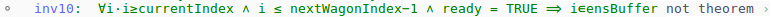
\includegraphics[scale=0.5]{../images/invariant.png}

Celui-ci est supposé garantir que l'ensemble compris dans le buffer est bien les indices compris entre ``currentIndex'' et ``nextWagonIndex''.
